\chapter{Simulation results}

In this chapter we present the results obtained to validate the numerical performance of the discretization method described in the previously chapters, compared with a reference simulation tool (SDEVICE \textcolor{red}{ref}). Moreover we describe (and compare) the algorithm used to calculate the current at contacts.

\section{Test cases}

We consider three kind of semiconductor devices: 

\begin{itemize}
\item {\bf p-n junction}
\item {\bf p-n junction in oxide}
\item {\bf MOSFET n-channel / p-channel}
\end{itemize}

\subsection{p-n junction}
\label{sec: PN}

In this example we consider a simple p-n junction. \figref{fig: diodo struttura} presents the partition used and the doping profile of this test case. The section of the parallelepiped is a $0.05 \times 0.05 [\mu m^2]$ square while the device is $0.1 [\mu m]$ long.  The number of verticises are $4933$, while the elements are $24576$.  The doping concentration is obtained setting a constant profile of acceptors over all the domain ($N_A = 1.0\times 10^{17}$) overhelmed by a doping profile of  donors ($N_D=1.0 \times 10^{18}$) bounded on one side of the device resulting in an almost abrupt junction. 
Two contacts are defined: (A) contact is placed at $Z=0.1[\mu m]$ and (B) contact is placed at $Z=0.0 [\mu m]$.  


\begin{figure}[!t]
\centering
\subfloat[][\emph{Mesh}]
{\includegraphics[height=3.5cm]{Results/DIODE/AAA_structureandcontactFINITO.png}}
\hspace{1cm}
\subfloat[][\emph{Doping concentration}]
{\includegraphics[height=3.5cm]{Results/DIODE/AAADopingConcentrationFINITO.png}}
\label{fig: diodo struttura}
\end{figure}


We proceed in order to analyze the operating function of the diode, therefore two cases in direct polarization are performed. The setting values and the parameters are summerized in \ref{tab: diode direct}. 




\figref{fig: Solutions case test 0.3} and \figref{fig: Solutions case diode 1V} report the behaviour of the solutions along a line parallel to the Z-axis and placed at the center of the device. 

Because the built-in voltage is around $0.7 \div 0.8 [V]$ the behaviour of the device is different when the applied bias is below or above the built-in voltage. 
At $0.3[V]$ of polarization potential drop is almost bounded around the junction, and due to the asymmetric doping, is major extended in the p-side. The carriers can't easily cross the potential barrier and this will cause a low current flux inside the device.
At $1.0[V]$ the minority carriers density becomes almost ten order bigger, resulting in a large ammount of current toward the contacts:  the device turns from exponential to linear resistive. This is clear in \figref{fig: diode 1v pot} where the potential shape becomes similar to a resistence voltage profile.  

Comparing the quasi-fermi potential of \figref{fig: qf pot diode 03} and \figref{fig: qf pot diode 1} the boundary layers at contacts increase with the polarization. This effect is related to the ohmic contact hypotesis, and can be avoided with different boundary condition, this occurs also for the carrier concentration because at the contacts the charge neutrality and the thermodynamic equilibrium  are imposed.

\figref{fig: diode potential 03V}$\div$\ref{fig: pdensity 03V} shows the comparison between SDEVICE and FEMOS in 3D plots for electrostatic potential, electron and hole densities for bias at $0.3[V]$, while \figref{fig: diode potential 1V}$\div$\ref{fig: pdensity 1V} show the shape comparison for bias at $1.0[V]$. In both of the condition the agreement is very good.


\begin{figure}[!h]
\centering

\subfloat[][\emph{Potential}]
{\includegraphics[height=4.5cm]{DatiImmaginiTESI/Diode/PotentialZaxis03volt.eps}}
\subfloat[][\emph{Potential} \label{fig: diode 1v pot}]
{\includegraphics[height=4.5cm]{DatiImmaginiTESI/Diode/PotentialZaxis1volt.eps}}


\subfloat[][\emph{Carriers}]
{\includegraphics[height=4.5cm]{DatiImmaginiTESI/Diode/DensitiesZaxis03volt.eps}}
\subfloat[][\emph{Carriers}]
{\includegraphics[height=4.5cm]{DatiImmaginiTESI/Diode/DensitiesZaxis1volt.eps}}


\subfloat[][\emph{Quasi fermi potential} \label{fig: qf pot diode 03}]
{\includegraphics[height=4.5cm]{DatiImmaginiTESI/Diode/QuasiFermiZaxis03volt.eps}}
\subfloat[][\emph{Quasi fermi potential} \label{fig: qf pot diode 1}]
{\includegraphics[height=4.5cm]{DatiImmaginiTESI/Diode/QuasiFermiZaxis1volt.eps}}

\caption{Solutions case test diode $V=0.3[V]$.}
\label{fig: Solutions case test 0.3}
\end{figure}

\begin{table}[!h]
\centering
\begin{tabular}{ccccc}
\toprule
 Test case & Mobility model & R/G model & $\epsilon_{Si}$ & $\epsilon_{0x}$  \\
\midrule
$V_A=0.3 [V]$ & $\mu_n = 1417$, $\mu_p = 470.5$ & SRH, Auger & 11.6 & - \\
$V_A=1.0 [V]$ & $\mu_n = 1417$, $\mu_p = 470.5$ & SRH, Auger & 11.6 & - \\\bottomrule
\end{tabular}
\caption{p-n junction - list of parameters.}
\label{tab: diode direct}
\end{table}



\clearpage 

\begin{figure}[!h]
\centering
\subfloat[][\emph{FEMOS}]
{\includegraphics[height=3.7cm]{Results/DIODE/FEMOS1817_potential03volt.png}}
\hspace{1cm}
\subfloat[][\emph{SDEVICE}]
{\includegraphics[height=3.7cm]{Results/DIODE/SDEVICE1817_potential03voltONLYDEVICE.png}}
\caption{p-n junction 0.3[V] - Potential.}
\label{fig: diode potential 03V}
\end{figure}

\vspace{1cm}

\begin{figure}[!h]
\centering
\subfloat[][\emph{FEMOS}]
{\includegraphics[height=3.7cm]{Results/DIODE/FEMOS1817_edensity03volt.png}}
\hspace{1cm}
\subfloat[][\emph{SDEVICE}]
{\includegraphics[height=3.7cm]{Results/DIODE/SDEVICE1817_edensity03voltONLYDEVICE.png}}
\caption{p-n junction 0.3[V] -  Electron density.}
\label{fig: ndensity 03V}
\end{figure}

\vspace{1cm}

\begin{figure}[!h]
\centering
\subfloat[][\emph{FEMOS}]
{\includegraphics[height=3.7cm]{Results/DIODE/FEMOS1817_hdensity03volt.png}}
\hspace{1cm}
\subfloat[][\emph{SDEVICE}]
{\includegraphics[height=3.7cm]{Results/DIODE/SDEVICE1817_hdensity03voltONLYDEVICE.png}}
\caption{p-n junction 0.3[V] - Hole density.}
\label{fig: pdensity 03V}
\end{figure}


\clearpage

\begin{figure}[!h]
\centering
\subfloat[][\emph{FEMOS}]
{\includegraphics[height=3.7cm]{Results/DIODE/FEMOS1817_potential1voltONLYDEVICE.png}}
\hspace{0.7cm}
\subfloat[][\emph{SDEVICE}]
{\includegraphics[height=3.7cm]{Results/DIODE/SDEVICE1817_potential1volt.png}}
\caption{p-n junction 1.0[V] - Potential.}
\label{fig: diode potential 1V}
\end{figure}

\vspace{1cm}

\begin{figure}[!h]
\centering
\subfloat[][\emph{FEMOS}]
{\includegraphics[height=3.7cm]{Results/DIODE/FEMOS1817_edensity1voltLINEARONLYDEVICE.png}}
\hspace{0.7cm}
\subfloat[][\emph{SDEVICE}]
{\includegraphics[height=3.7cm]{Results/DIODE/SDEVICE1817_edensity1voltLINEARWITHLEGEND.png}}
\caption{p-n junction 1.0[V] -  Electron density.}
\label{fig: ndensity 1V}
\end{figure}

\vspace{1cm}

\begin{figure}[!h]
\centering
\subfloat[][\emph{FEMOS}]
{\includegraphics[height=3.7cm]{Results/DIODE/FEMOS1817_hdensity1voltLINEARONLYDEVICE.png}}
\hspace{0.7cm}
\subfloat[][\emph{SDEVICE}]
{\includegraphics[height=3.7cm]{Results/DIODE/SDEVICE1817_hdensity1voltLINEARWITHLEGEND.png}}
\caption{p-n junction 1.0[V] - Hole density.}
\label{fig: pdensity 1V}
\end{figure}

\clearpage

\subsubsection{Computational cost and initial condition}

It's well known that the convergence time is strictly related to the kind of initial condition on device. However predict in every situations the possibly shape of the solutions is hard, if not even impossible. For this reason we have adopted a common and general approach splitting the domain in several regions accordingly to their doping concentration: each of the semiconductor regions are treated as they are in equilibrium with the nearest contact then the guess value for $\varphi$ is obtained thanks to the relations \referenzaeq{eq: non eq n density mb} or \referenzaeq{eq: non eq p density mb}. 

It's quite simple implement this kind of initial profile and it's reasonable thinking that for solutions near the equilibrium this method will guarantee good converging performances. 

In order to analyze the response of the system at different bias an additional case test is proposed. In the range between $0.0[V]$ and $3.0[V]$ several voltages were applied on the previous device. For every bias point the initial guess is computed with the above mentioned way. 

\figref{fig: tempi computazionali 1} shows how the computational cost of computing the solution increases with the increasing of the applied bias. Moreover as expected if the mesh is finer the time needed to find the solution increases, resulting in a rigid shift of the curve toward high time value.


\begin{figure}[!b]
\centering
\includegraphics[height=7cm]
{Results/Caratteristiche/Diode/ComputationalTimeDifferentMeshes.eps}
\caption{Total time Gummel Map.}
 \label{fig: tempi computazionali 1}
 \end{figure}
 
 
Focusing on the case test related to the coarser mesh additional considerations may be done. In \figref{fig: tempi computazionali 2} it's evident how the average time spent to solve the NLP and the DD equations remains almost unchanged. On the contrary the number of GM iterations needed by the system to reach the solution, increases for voltages above $1.5[V]$.

A reasonable explanation of this phenomenon could be found comparing solution and initial guess for a bias below and above $1.5[V]$ (similar considerations may be done if we consider the carrier densities). When voltage is low, like in \figref{fig: different biast initial step 1} ($V_A = 0.1[V]$), the potential shape is well predicted by the initial guess, resulting easier for the Gummel map converging toward the solution. On the contrary in \figref{fig: different biast initial step 2} ($V_A=1.6[V]$) the device operates as a resistence and the potential profile seems more to a linear function, this implies that from an initial condition of equilibrium the algorithm have to spent more steps in order to reach the solution. 


 
 \begin{figure}[!t]
\centering
\includegraphics[height=7cm]{Results/Caratteristiche/Diode/ConfrontoTempiNLPDDGMiterations.eps}
\caption{Time NLP and DD, iteration GM.}
\label{fig: tempi computazionali 2}
\end{figure}

\begin{figure}[!b]
\centering
\subfloat[][\label{fig: different biast initial step 1}]
{\includegraphics[height=4.5cm]{DatiImmaginiTESI/Diode/PotentialZaxis01volt.eps}}
\subfloat[][\label{fig: different biast initial step 2}]
{\includegraphics[height=4.5cm]{DatiImmaginiTESI/Diode/PotentialZaxis15volt.eps}}
\caption{Initial step for different bias.}
\label{fig: different biast initial step}
\end{figure}
 



\clearpage


\subsection{p-n junction in oxide}
\label{sec: PNOX}

In this test case a silicon p-n junction of $0.3[\mu m]$ long has been surrounded by an oxide layer of $0.025[\mu m]$ thick. The section of the slicon part is a $0.1 \times 0.1 [\mu m^2]$ square.  We spent $6334$ verticies overall the domain \textcolor{red}{elements}. The structure and the doping are well defined in \figref{fig: structure diodeox}. The setting of the electrode is similar to the previously test case and contacts are defined only on silicon surface. 
\tabref{tab: diodeox 3d} reports the models and parameters used.

\figref{fig: plot 1D diodeox} reports the behaviour of the solutions and the quasi fermi potential levels along a line parallel to the Z-axis and placed at the center of the device. The main features are similar to the previous device, indeed notice the boundary layers at contact for the carrier densities and the quasi fermi potential levels.
\figref{fig: potential diodeox} $\div$ \ref{fig: hdensity diodeox} show the 3D solutions for the case at $0.3[V]$, while \figref{fig: potential diodeox 1V}$\div$\ref{fig: hdensity diodeox 1V} refer to the case at $1.0[V]$. Both in 1D and 3D comparison charts the agreement with the commercial software is good. 

\vspace{0.5cm}

\begin{figure}[!h]
\centering
\subfloat[][\emph{Mesh}]
{\includegraphics[height=4.5cm]{Results/DIODEOX/AAA_structureandcontact2.png}}
\hspace{1.5cm}
\subfloat[][\emph{Doping concentration}]
{\includegraphics[height=4.5cm]{Results/DIODEOX/AAA_Dopingconcentration2ONLYDEVICE.png}}
\caption{Test case p-n junction in oxide.}
\label{fig: structure diodeox}
\end{figure}


\vspace{0.5cm}

\begin{table}[!h]
\centering
\begin{tabular}{ccccc}
\toprule
 Test case & Mobility model & R/G model & $\epsilon_{Si}$ & $\epsilon_{0x}$  \\
\midrule
$V_A=0.3 [V]$ & $\mu_n = 1417$, $\mu_p = 470.5$ & SRH, Auger & 11.6 & 3.9 \\
$V_A=1.0 [V]$ & $\mu_n = 1417$, $\mu_p = 470.5$ & SRH, Auger & 11.6 & 3.9 \\\bottomrule
\end{tabular}
\caption{List of parameters.}
\label{tab: diodeox 3d}
\end{table}




\begin{figure}[!t]
\centering

\subfloat[][\emph{Electrostatic potential.}]
{\includegraphics[height=4.6cm]{DatiImmaginiTESI/DiodeOx/PotentialZaxis.eps}}
\subfloat[][\emph{Electrostatic potential.}]
{\includegraphics[height=4.6cm]{DatiImmaginiTESI/DiodeOx/PotentialZaxis1VOLT.eps}}


\subfloat[][\emph{Hole and electron densities.}]
{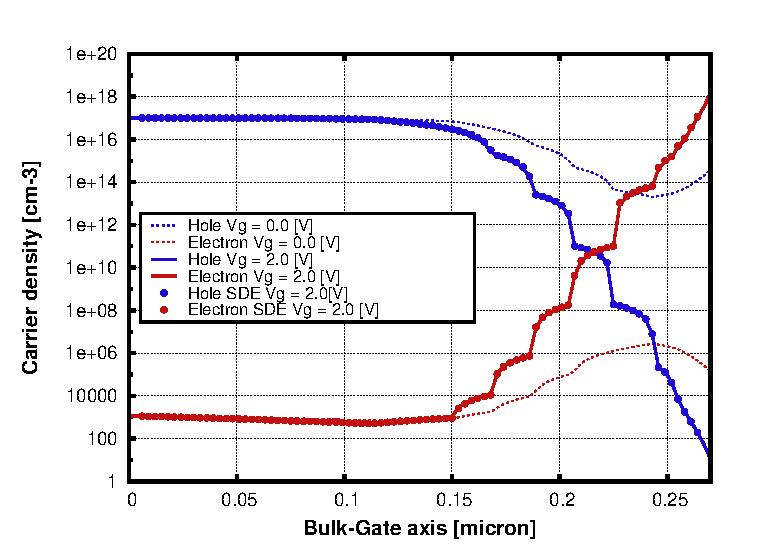
\includegraphics[height=4.6cm]{DatiImmaginiTESI/DiodeOx/DensityZaxis.eps}}
\subfloat[][\emph{Hole and electron densities.}]
{\includegraphics[height=4.6cm]{DatiImmaginiTESI/DiodeOx/DensityZaxis1VOLT.eps}}


\subfloat[][\emph{Quasi fermi potential levels.}]
{\includegraphics[height=4.6cm]{DatiImmaginiTESI/DiodeOx/QFPotentialZaxis.eps}}
\subfloat[][\emph{Quasi fermi potential levels.}]
{\includegraphics[height=4.6cm]{DatiImmaginiTESI/DiodeOx/QFPotentialZaxis1VOLT.eps}}


\caption{Plots of the solutions and the quasi fermi potential levels along the line parallel to the Z-axis and placed at the center of the device. On the left is presented the test case at $V_a=0.3[V]$ while on the left at $V_A=1.0[V]$.}
\label{fig: plot 1D diodeox}
\end{figure}

\clearpage


\begin{figure}[!h]
\centering
\subfloat[][\emph{FEMOS}]
{\includegraphics[height=4.5cm]{Results/DIODEOX/FEMOS1817_potential03volt.png}}
\hspace{1cm}
\subfloat[][\emph{SDEVICE}]
{\includegraphics[height=4.5cm]{Results/DIODEOX/SDEVICE1817_potential03voltONLYDEVICE.png}}
\caption{p-n junction in oxide 0.3[V] - Potential.}
\label{fig: potential diodeox}
\end{figure}

\vspace{0.5cm}

\begin{figure}[!h]
\centering
\subfloat[][\emph{FEMOS}]
{\includegraphics[height=4.5cm]{Results/DIODEOX/FEMOS1817_edensity03volt.png}}
\hspace{1cm}
\subfloat[][\emph{SDEVICE}]
{\includegraphics[height=4.5cm]{Results/DIODEOX/SDEVICE1817_edensity03voltONLYDEVICE.png}}
\caption{p-n junction in oxide 0.3[V] - Electron density.}
\label{fig: edensity diodeox}
\end{figure}

\vspace{0.5cm}

\begin{figure}[!h]
\centering
\subfloat[][\emph{FEMOS}]
{\includegraphics[height=4.5cm]{Results/DIODEOX/FEMOS1817_hdensity03volt.png}}
\hspace{1cm}
\subfloat[][\emph{SDEVICE}]
{\includegraphics[height=4.5cm]{Results/DIODEOX/SDEVICE1817_hdensity03voltONLYDEVICE.png}}
\caption{p-n junction in oxide 0.3[V] - Hole density.}
\label{fig: hdensity diodeox}
\end{figure}

\clearpage


\begin{figure}[!h]
\centering
\subfloat[][\emph{FEMOS}]
{\includegraphics[height=4.5cm]{Results/DIODEOX/FEMOS1817_potential1voltONLYDEVICE.png}}
\hspace{1cm}
\subfloat[][\emph{SDEVICE}]
{\includegraphics[height=4.5cm]{Results/DIODEOX/SDEVICE1817_potential1voltONLYDEVICE.png}}
\caption{p-n junction in oxide 1.0[V] - Potential.}
\label{fig: potential diodeox 1V}
\end{figure}

\vspace{0.5cm}

\begin{figure}[!h]
\centering
\subfloat[][\emph{FEMOS}]
{\includegraphics[height=4.5cm]{Results/DIODEOX/EdensityLINEARDIODEOXONLYDEVICE.png}}
\hspace{1cm}
\subfloat[][\emph{SDEVICE}]
{\includegraphics[height=4.5cm]{Results/DIODEOX/EdensityLINEARDIODEOXONLYDEVICEsde.png}}
\caption{p-n junction in oxide 1.0[V] - Electron density.}
\label{fig: edensity diodeox 1V}
\end{figure}

\vspace{0.5cm}

\begin{figure}[!h]
\centering
\subfloat[][\emph{FEMOS}]
{\includegraphics[height=4.5cm]{Results/DIODEOX/HdensityLINEARDIODEOXONLYDEVICE.png}}
\hspace{1cm}
\subfloat[][\emph{SDEVICE}]
{\includegraphics[height=4.5cm]{Results/DIODEOX/HdensityLINEARDIODEOXONLYDEVICEsde.png}}
\caption{p-n junction in oxide 1.0[V] - Hole density.}
\label{fig: hdensity diodeox 1V}
\end{figure}

\clearpage





\subsubsection{3D effect of the electric field}


Looking at \figref{fig: potential diodeox} it's clear that for low bias the electrostatic potential behaves differently in the two materials.
This phenomena could be explained if we think about the relation \referenzaeq{eq: relazione pot electric} between electric field and potential.
In fact, as we imposed $\nabla \varphi \cdot \vect{n}=0$ on the oxide boundary no field lines of the electric field could cross that boundary. The consequence is that all the field lines could start and end only from the contact A or B.
Polarization can't operate directly on the oxide and the behaviour of the the electric field inside the device is due only to the displacement effect in the junction of the silicon, which imposes the electric response in the oxide material. \figref{fig: electric field diode} reports the field lines of the electric field in the case $V_A=0.3[V]$ comparing with the commercial software. The visible effect is a lower magnitude of the electric field in the oxide, resulting a more diffused potential.

This phenomena seems to disappear for high bias: in \figref{fig: potential diodeox 1V} the influence of the contact (A) becomes much higher and the electorstatic potential tends to conform over the entire domain.



\begin{figure}[!h]
\centering
\subfloat[][\emph{FEMOS}]
{\includegraphics[height=4.7cm]{Results/DIODEOX/FEMOS1817_electricfield03volt.png}}
\hspace{1.5cm}
\subfloat[][\emph{SDEVICE}]
{\includegraphics[height=4.7cm]{Results/DIODEOX/SDEVICE1817_electricfield03voltONLYDEVICE.png}}
\caption{Test case dide p-n in ox 0.3[V], electric field.}
\label{fig: electric field diode}
\end{figure}






It is important to note that displacment approach doesn't satisfied  in a strong manner the pricinple of action and reaction.
This is equivalent to say that given two element $K_i,K_j\in \mathcal{T}_h$ such that $K_i \bigcap K_j = f_i$ where $f_i \in \mathcal{F}_h$ and let be  $\vect{n}_{i}$ the outward normal vector of $\partial K_i$ and $\vect{n}_{j}$ the outward normal vector of $\partial K_j$,  we ensure the following equations only in a weak way

\begin{align}
\vect{D}|_{K_i}\cdot \vect{n}_{i} & = \vect{D}|_{K_j} \cdot \vect{n}_{j} \label{eq: conservazione vettore spostamento}\\
\vect{J}_n|_{K_i}\cdot \vect{n}_{i} & = \vect{J}_n|_{K_j}\cdot \vect{n}_{j} \\
\vect{J}_p|_{K_i}\cdot \vect{n}_{i} & = \vect{J}_p|_{K_j}\cdot \vect{n}_{j} 
\end{align}


In fact taking in consideration equation \referenzaeq{eq: conservazione vettore spostamento}, we can state that along the interface silicon-oxide the following equality holds

\begin{equation}
\epsilon_{ox}\vect{E}|_{K_i}\cdot \vect{n}_{i} = \epsilon_{Si}\vect{E}|_{K_j} \cdot \vect{n}_{j} \psp{5} \Rightarrow \psp{5}  [\vect{E}|_{K_i}]_y = \dfrac{\epsilon_{Si}}{\epsilon_{ox}}[\vect{E}|_{K_j}]_y
\end{equation}  

Accordingly with the parameters used during the simulations $\epsilon_{Si}/\epsilon_{ox}=2.97$, which means that the normal component on the interface of the electric field has a gap passing from oxide to semicondctor and vice versa. \figref{fig: salto electric field} shows a plots of $E_y$ along a line parallel to the Y-axis which crosses both oxide and silicon material. For this setting $E_y\equiv\vect{E}\cdot \vect{n}$ on the interface and the drop of magnitude is quite visible. The ratio between the two interfaces is almost $3.8$ for both $y=0.05[\mu m]$ and $y = 0.15[\mu m]$.
This example really shows the effect of the phenomena we mentionend before and the consequence which the solutions could own.

 Furthermore every tetrahedral interfaces of the partition are affected by this problem, which means that inside an omogenous material the normal component of the electric field doesn't conserve from one element of the grid to the neighbouring ones. Even the presence of this drawback, the solutions obtained are good, but if you would satisfy equation \referenzaeq{eq: conservazione vettore spostamento} in a strong manner you need to move for mixed-hibryd formulation \textcolor{red}{ref} which ensures the conservation of the flux even under possbile strong discontinuities of material properties.


\begin{figure}[!h]
\centering
\includegraphics[height=5cm]{DatiImmaginiTESI/DiodeOx/ElectricFieldYaxis.eps}
\caption{$E_y$ along a line parallel to Y-axis, $z=0.22[\mu m]$ and $x=0.1[\mu m]$.}
\label{fig: salto electric field}
\end{figure}


\clearpage





\subsection{MOSFET n-channel}
\label{sec: MOS}


The description of MOSFET device can be found in \cite{ModernVLSIdevices}: it is a four-terminal device with the electrodes designeted as gate (G), source (S), drain (D) and substrate or bulk (B). The gate electrode is usually made of metal or heavily doped polysilicon and is separated from the substrate by a thin silicon dioxide. The surface region under the gate  oxide between source and drain is called the \textit{channel} region.
Because the current in a MOSFET is transported predominantly by carriers of one polarity, the MOSFET is usually referred to as a unipolar or majority-carrier device, as a propose of test we consider a n-channel (n-MOSFET) or a p-channel (p-MOSFET). An \textit{n-MOSFET} (p-MOSFET) consists of a p-type (n-type) silicon substrate into which two n-regions (p-regions) are the designing source and drain. The n-regions (p-regions) are doped accordingly with a gaussain profile as occuring from an implantation. 
\figref{fig: mos geometry 1} and \figref{fig: mos geometry 2} shows the geometry and the doping concentration for n-MOSFET and p-MOSFET respectively. 
We note that the mesh has been refined where the more interesting phenomena occur: along channel and over the deplation regions.

When no voltage is applied to the gate, no current flows between the source and drain, while if a sufficiently large positive voltage is applied to the gate, the silicon surface is inverted to n-type (p-type), which forms a conducting channel between the source and drain: applying a positive voltage to the drain (source) the electrons (holes) start to flow from source to drain and therefore a current is generated. 

\begin{figure}[!b]
\centering
\subfloat[][\emph{Mesh}\label{fig: mos geometry 1}]
{\includegraphics[height=4.2cm]{Results/MOS/AAA_MeshAndContact.png}}
\hspace{0.5cm}
\subfloat[][\emph{Doping concentration}\label{fig: mos geometry 2}]
{\includegraphics[height=4.2cm]{Results/MOS/AAA_DopingConcentrationONLYDEVICE.png}}
\caption{Geometry of the test case MOS n-channel.}
\label{fig: mos geometry}
\end{figure}




The explanation of the MOSFET working principle has ben clarified in \figref{fig: energy levels MOS} where for the case of n-channel the band profile along the channel axis has been reported for two different gate bias.
The voltage applyed to the gate tends to decrease the flow of the electron as the energy barrier doesn't exist anymore.
\figref{fig: channel figures 1D} shows for an n-channel the profile of carrier concentrations in the middle of the channel cut perpendicular to the gate, for off-state and on-state: the inversion occurs when the gate voltage is higher than MOSFET threshold.
The voltage applyed to the gate tends to decrease the band levels in the channel region: in this configuration the drain voltage causes the flow of the electron as the energy barrier doesn't exist anymore (see \figref{fig: energy levels MOS}).
\figref{fig: channel figures 3D} shows the 3D view of the n-channel space charge after inversion.



\begin{figure}[!t]
\centering
\subfloat[][\emph{$V_G=0.0[V]$, $V_D=0.1[V]$}]
{\includegraphics[scale=0.55]{DatiImmaginiTESI/Mos/BandDiagramMOS0volt.eps}}
\subfloat[][\emph{$V_G=2.0[V]$, $V_D=0.1[V]$}]
{\includegraphics[scale=0.55]{DatiImmaginiTESI/Mos/BandDiagramMOS2volt.eps}}
\caption{Energy band levels.}
\label{fig: energy levels MOS}
\end{figure}



The parameters and models used for these simulations are summerized in \tabref{tab: mos direct pol}. \figref{fig: potential mos off}$\div$\ref{fig: pdensity mos off} shows the 3D components of the electrostatic potential, electron density and hole density between the FEMOS results and the commercial code for the off-state MOSFET, while \figref{fig: potential mos}$\div$\ref{fig: pdensity mos} for the on-state MOSFET: the agreement is very good.


\begin{figure}[!b]
\centering
\subfloat[][1D cut perpendicular to the channel. \label{fig: channel figures 1D}]
{\includegraphics[height=4.5cm]{DatiImmaginiTESI/Mos/DensityZaxis.eps}}
\hspace{1cm}
\subfloat[][Space charge.\label{fig: channel figures 3D}]
{\includegraphics[height=4.5cm]{Results/PlotOverLine/Mos/Contour3DSpacechargeONLYDEVICE}}
\caption{Channel formation of the nMOSFET.}
\label{fig: channel figures}
\end{figure}


Finally \figref{fig: electric field mos} reports the streamline plot of the electric field inside the device for FEMOS and the SDEVICE:
\textcolor{red}{????}

\begin{figure}[!h]
\centering
\subfloat[][\emph{FEMOS}]
{\includegraphics[height=4.5cm]{Results/MOS/FEMOS181718_ElectricField2voltONLYDEVICE.png}}
\hspace{0.5cm}
\subfloat[][\emph{SDEVICE}]
{\includegraphics[height=4.5cm]{Results/MOS/SDEVICE181718_ElectricField2voltONLYDEVICE.png}}
\caption{Electric field density - $V_G = 2.0 [V]$.}
\label{fig: electric field mos}
\end{figure}

\vspace{0.5cm}



\begin{table}[!h]
\centering
\begin{tabular}{ccccc}
\toprule
 Test case & Mobility model & R/G model & $\epsilon_{Si}$ & $\epsilon_{0x}$  \\
\midrule
 $V_G=0.0 [V]$, $V_D=0.0[V]$,& $\mu_n = 1417$ & \multirow{2}*{SRH, Auger, II} & \multirow{2}*{11.6} & \multirow{2}*{3.9} \\
 $V_S=V_B=0.0[V]$ & $\mu_p = 470.5$ & & & \\ 
\midrule
$V_G=2.0 [V]$, $V_D=0.1[V]$,& $\mu_n = 1417$ & \multirow{2}*{SRH, Auger} & \multirow{2}*{11.6} & \multirow{2}*{3.9} \\
 $V_S=V_B=0.0[V]$ & $\mu_p = 470.5$ & & & \\
 \bottomrule
\end{tabular}
\caption{List of parameters.}
\label{tab: mos direct pol}
\end{table}

\clearpage

\begin{figure}[!h]
\centering
\subfloat[][\emph{FEMOS}]
{\includegraphics[height=4.4cm]{Results/MOS/MOSNelectrostaticpotSUBTHRESONLYDEVICE.png}}
\hspace{0.8cm}
\subfloat[][\emph{SDEVICE}]
{\includegraphics[height=4.4cm]{Results/MOS/MOSNelectrostaticpotSUBTHRESwithlegend.png}}
\caption{Electrostatic potential - $V_G = 0.0 [V]$.}
\label{fig: potential mos off}
\end{figure}

\vspace{0.5cm}

\begin{figure}[!h]
\centering
\subfloat[][\emph{FEMOS}]
{\includegraphics[height=4.4cm]{Results/MOS/MOSNedensitySUBTHRESONLYDEVICE.png}}
\hspace{0.8cm}
\subfloat[][\emph{SDEVICE}]
{\includegraphics[height=4.4cm]{Results/MOS/MOSNedensitySUBTHRESwithlegend.png}}
\caption{Electron density - $V_G = 0.0 [V]$.}
\label{fig: ndensity mos off}
\end{figure}

\vspace{0.5cm}

\begin{figure}[!h]
\centering
\subfloat[][\emph{FEMOS}]
{\includegraphics[height=4.4cm]{Results/MOS/MOSNhdensitySUBTHRESONLYDEVICE.png}}
\hspace{0.8cm}
\subfloat[][\emph{SDEVICE}]
{\includegraphics[height=4.4cm]{Results/MOS/MOSNhdensitySUBTHRESwithlegend.png}}
\caption{Electron density - $V_G = 0.0 [V]$.}
\label{fig: pdensity mos off}
\end{figure}






\clearpage

\begin{figure}[!h]
\centering
\subfloat[][\emph{FEMOS}]
{\includegraphics[height=4.5cm]{Results/MOS/FEMOS181718_potential2voltONLYDEVICE.png}}
\hspace{0.8cm}
\subfloat[][\emph{SDEVICE}]
{\includegraphics[height=4.5cm]{Results/MOS/SDEVICE181718_potential2voltONLYDEVICE.png}}
\caption{Electrostatic potential - $V_G = 2.0 [V]$.}
\label{fig: potential mos}
\end{figure}

\vspace{0.5cm}

\begin{figure}[!h]
\centering
\subfloat[][\emph{FEMOS}]
{\includegraphics[height=4.5cm]{Results/MOS/FEMOS181718_ndensity2voltONLYDEVICE.png}}
\hspace{0.8cm}
\subfloat[][\emph{SDEVICE}]
{\includegraphics[height=4.5cm]{Results/MOS/SDEVICE181718_ndensity2voltONLYDEVICE.png}}
\caption{Electron density - $V_G = 2.0 [V]$.}
\label{fig: ndensity mos}
\end{figure}

\vspace{0.5cm}

\begin{figure}[!h]
\centering
\subfloat[][\emph{FEMOS}]
{\includegraphics[height=4.5cm]{Results/MOS/FEMOS181718_pdensity2volt.png}}
\hspace{0.8cm}
\subfloat[][\emph{SDEVICE}]
{\includegraphics[height=4.5cm]{Results/MOS/SDEVICE181718_pdensity2voltONLYDEVICE.png}}
\caption{Electron density - $V_G = 2.0 [V]$.}
\label{fig: pdensity mos}
\end{figure}




\subsubsection{Inverse polarization}
\label{sec: inv pol mos}

In section \ref{sec: continuity equations} we pointed that the discretization scheme (EAFE) can't satisfy the discrete maximum principle in 3D simulations unless we satisfy condition  \referenzaeq{eq: mesh delaunay condition}.  Therefore it is possible encounter negative solution and we usually have to deal with this problem when the concentration of electrons and holes become low.

In order to hilight this possible critical situation n-channel MOSFET has put in inverse polarization by grounded all contacts except the drain: ramped to $0.5[V]$.

\figref{fig: negative carriers MOS} reports the solutions of the electron density computed with FEMOS and SDEVICE using the meshe presented in \figref{fig: mos geometry 2}: the results are comparable, but near the drain-bulk junction the FEMOS solution presents some points with negative concentrations. Increasing drain bias  the phenomenon will tend to spread over a larger area, untill it affects irremediably the computation.
The most practice technique to avoid this problem is the fitting of the mesh around the problematic regions.
\figref{fig: drain stress mos 13000 1} represents a more fine mesh with $13000$ points and $67388$ elements. Using this mesh the correctness of the solution is recovered \figref{fig: drain stress mos 13000 2}. \figref{fig: zikatanov mos} shows how the satisfaction of condition \referenzaeq{eq: mesh delaunay condition} changes between the different meshes used: increasing the number of degree of freedom over the critical region guarantees a better fulfillment of \referenzaeq{eq: mesh delaunay condition}. 

In order to treat this situation it may be useful implement suitable a-posteriori error estimation and adaptive mesh refinement techniques \textcolor{red}{ref.}. 

Finally \figref{fig: pot MOS negative} and \figref{fig: hole MOS negative} presents the solution of electrostatic potential and hole density computed on the finer mesh and compared with the commercial tool: also for that quantitaty the agreement is good.

\begin{table}[!h]
\centering
\begin{tabular}{ccccc}
\toprule
 Test case & Mobility model & R/G model & $\epsilon_{Si}$ & $\epsilon_{0x}$  \\
\midrule
 $V_G=0.0 [V]$, $V_D=0.5[V]$,& $\mu_n = 1417$ & \multirow{2}*{SRH, Auger, II} & \multirow{2}*{11.6} & \multirow{2}*{3.9} \\
 $V_S=V_B=0.0[V]$ & $\mu_p = 470.5$ & & & \\ 
 \bottomrule
\end{tabular}
\caption{List of parameters.}
\end{table}


\begin{figure}[!h]
\centering

\subfloat[][\emph{FEMOS}]
{\includegraphics[height=4.4cm]{Results/Drainstress/MOSNelectrostaticpotDRAINSTRESSONLYDEVICE.png}}
\hspace{1cm}
\subfloat[][\emph{SDEVICE}]
{\includegraphics[height=4.4cm]{Results/Drainstress/MOSNelectrostaticpotDRAINSTRESSwithlegend.png}}

\caption{Electrostatic potential - Inverse polarization.}
\label{fig: pot MOS negative}
\end{figure}


\begin{figure}[!h]

\subfloat[][\emph{FEMOS}]
{\includegraphics[height=4.4cm]{Results/Drainstress/MOSNhdensityDRAINSTRESSONLYDEVICE.png}}
\hspace{1cm}
\subfloat[][\emph{SDEVICE}]
{\includegraphics[height=4.4cm]{Results/Drainstress/MOSNhdensityDRAINSTRESSwithlegend.png}}

\caption{Hole density - Inverse polarization.}
\label{fig: hole MOS negative}
\end{figure}

\clearpage 



\begin{figure}[!h]
\centering
\subfloat[][\emph{FEMOS}]
{\includegraphics[height=4.3cm]{Results/Drainstress/NegativeCarrierOnlydevice.png}}
\hspace{1cm}
\subfloat[][\emph{SDEVICE}]
{\includegraphics[height=4.3cm]{Results/Drainstress/CarrierSDEonlydevicewithlegend.png}}
\caption{Negative carriers in the electron density solution.}
\label{fig: negative carriers MOS}
\end{figure}

\begin{figure}[!h]
\centering
\subfloat[][\emph{Mesh} \label{fig: drain stress mos 13000 1}]
{\includegraphics[height=4.3cm]{Results/Drainstress/MosMeshFitted.png}}
\hspace{1cm}
\subfloat[][\emph{FEMOS} \label{fig: drain stress mos 13000 2}]
{\includegraphics[height=4.3cm]{Results/Drainstress/NegativeCarrier13000withlegend.png}}
\caption{Test case with finer mesh.}
\label{fig: drain stress mos 13000}
\end{figure}

\begin{figure}[!h]
\centering
\subfloat[][\emph{Coarse mesh.}]
{\includegraphics[height=4cm]{Results/Drainstress/Zikatanov3000.png}}
\hspace{1cm}
\subfloat[][\emph{Fine mesh.}]
{\includegraphics[height=4cm]{Results/Drainstress/Zikatanov13000withlegend.png}}
\caption{Satisfaction of the Zikatanov condition.}
\label{fig: zikatanov mos}
\end{figure}

\clearpage


\section{Calculation of the current at contacts}

During the analysis of an electric device, one of the most useful information is the electrical response at terminals. In order to accomplish this target we have to compute the integral of the electron and hole current density over a generic 2D electrode. We report here the the procedure found in \cite{ContactCurrentRM} (\textit{residue method}) in the case of 3D: the analysis make is easiliy extendable to our case if we consider also the work \cite{GalerkMethConsHughes}. Moreover we remark that the method can be succesfully applied to a wide spread of applications, including contact charges, carrier quantum probability fluxes and heat fluxes.

A contact is defined by a surface and more precisely we can consider $\Gamma_{D,Si} = \bigcup_{c=1}^d \Gamma_c$ where $d$ is the number of terminals on the device and $\forall c=1,...,d$, $\Gamma_c$ is the $c$-th contact. For each contact we need to compute the total current $I_c$ as:

\begin{equation}
\mathcal{I}_c = \mathcal{I}_c^n + \mathcal{I}_c^p
\end{equation}

where $\mathcal{I}_c^n$ is the contribution of the electron current and $\mathcal{I}_c^p$ is the contribution of the hole current.
For a given contact $\Gamma_c$, the fluxes of the current density assume the following form:

\begin{equation}
\label{eq: current flux}
\mathcal{I}_c^\nu = \int_{\Gamma_c}\vect{J}_\nu(\nu) \cdot \vect{n} \, d{\Gamma} \psp{10} \nu = \{n,p\}
\end{equation}

where as usual $\vect{n}$ is the unit outward normal of the domain boundary. It's well known that the evaluation of boundary integrals is a difficult task. Many difficulties in the numerical evalutaion of \referenzaeq{eq: current flux} arise from singularities in spatial derivatives of the approximate solution $n_h$ or $p_h$ near the contact edges, due to a change in the boundary condition type from Dirichlet to Neumann at the contact ends.



Consider the discretized electron continuity problem \referenzaeq{eq: weak formulation displacement} and let be $\eta$  the set of all vertices of the partition $\mathcal{T}_h$.  We can split the set of total nodes in contact node $\eta_g \in \Gamma_{D,Si}$ and the complementary part $\eta_n \in \Gamma_{N,Si}$. We define an \textit{auxiliary flux} $H_h$ on $\Gamma_{D,Si}$ as

\begin{equation}
H_h = \sum_{i\in\eta_g} H_{h,i} \psi_i 
\end{equation}


Now given the spaces:

\begin{align*}
\mathcal{V}_h = & span\{\psi_i\}_{i \in \eta_n} \\
\vect{V}_h = & span\{\psi_i\}_{i \in \eta_g}  \\
\mathcal{S}_h = & \{u \in \mathcal{V}_h \oplus \vect{V}_h: u|_{\Gamma_{D,Si}} = n_D \}
\end{align*}

it's possible write a modified form of Glakerin's method which reads as: 

find $n_h  \in \mathcal{S}_h$ and $H_h \in \vect{V}_h$ such that

\begin{equation}
\label{eq: modified galerkin}
(W_h,H_h)_{\Gamma_{D,Si}} = a(W_h,n_h)-F(W_h) \psp{10} \forall W_h \in \mathcal{V}_h \oplus \vect{V}_h
\end{equation}

where $a(\cdot,\cdot)$ is the bilinear form \referenzaeq{eq: weak formulation displacement} and $F(\cdot)$ the relative functional.
Equation \referenzaeq{eq: modified galerkin} splits into two subproblems:

\begin{align}
0  & = a(w_h,n_h)-F(w_h) \psp{10} \forall w_h \in \mathcal{V}_h \label{eq: usual problem}\\
(W_h,H_h)_{\Gamma_{D,Si}} & = a(W_h,n_h)-F(W_h) \psp{10} \forall W_h \in \vect{V}_h \label{eq: flux problem}
\end{align}

Problem \referenzaeq{eq: usual problem} is identical to the unmodified case and can be treated as before or using a different discretization scheme. Once obtained the solution $n_h$ problem \referenzaeq{eq: flux problem} is fully decoupled from \referenzaeq{eq: usual problem} and we can determines $H_h$ as follows

\begin{equation}
\label{eq: flux problem complete}
(H_h,\psi_i)_{\Gamma_{D,Si}} = a(\psi_i,n_h)-F(\psi_i) \psp{10} \forall i \in \eta_g 
\end{equation} 


\cite{GalerkMethConsHughes} demonstrates that $H_h$ defines the conserved total flux along $\Gamma_{D,Si}$ and accordingly with the boundary condition, the following equality is obtained

\begin{equation}
\label{eq: conservative flux}
\int_{\Gamma_{D,Si}} H_h \, d\Gamma = - \int_{\Omega_{Si}} qR \, d \Omega
\end{equation}


On the other hand if we apply the Divergence theorem on \referenzaeq{eq: LEC system} we can state 

\begin{equation}
\label{eq: lec divergence theor}
\int_{\Gamma_{D,Si}} \vect{J}_n \cdot \vect{n} \, d\Gamma = \int_{\Omega} - qR \, d\Omega
\end{equation}

Equation \referenzaeq{eq: conservative flux} and \referenzaeq{eq: lec divergence theor}  lead us to conclude that for all contacts holds

\begin{equation}
\label{eq: flux current formula}
\mathcal{I}_c^n = \int_{\Gamma_c} H_h \, d\Gamma
\end{equation}

In order to compute \referenzaeq{eq: flux current formula} let be $\eta_{c}$ the set of nodes of the contact $\Gamma_c$, the following equalities hold

\begin{equation}
\label{eq: equalities integrals}
\sum_{l \in \eta_c} \int_{\Gamma_c} H_h \psi_l \, d\Gamma 
=  \int_{\Gamma_c} H_h \sum_{l \in \eta_{c}} \psi_l \,d\Gamma 
= \int_{\Gamma_c} H_h \, d\Gamma
\end{equation}


Accordingly with  \referenzaeq{eq: equalities integrals} we can reinterpret $(H_h,\psi_i)_{\Gamma_{D,Si}}$ as the contribution to the flux at node $i$ and therefore the current at contact $c$ is given by summing over the verticies $\eta_{c}$ this quantity.

Therefore the residue method is:
given the system matrix $A$ of the Drif-Diffusion equation, the solution $n_h$ and the right hand side $\vect{b}$, $\forall c = 1,...,d$ the contribution to the total contact current is

\begin{equation}
\mathcal{I}_c^n = (An_h-\vect{b})\cdot \mathbb{I}_c
\end{equation} 

where

\begin{equation}
[\mathbb{I}_c]_i := \left\{ \begin{array}{ll}
0 & i \notin \eta_c \\
1 & i \in \eta_c
\end{array}  \right.
\end{equation} 

Obiouvsly the result is holds also for the hole continuity equation. 

%Let be $A$ the system matrix of the continuity equation \referenzaeq{eq: matrice continuità} and $\vect{b}$ the relative right hand side before applying boundary conditions.  The linear problem looks as:
%
%\begin{equation}
%\label{eq: discretization before bc}
%\sum_{j\in\eta} A_{ij} \nu_j = b_i \psp{10} \forall i \in \eta
%\end{equation}
%
%
%Notice that the values of $\nu_j$ are known on the contacts and \referenzaeq{eq: discretization before bc} can be rewritten as follows:
%
%\begin{equation}
%\label{eq: discretization before bc 2}
%\begin{cases}
%
%\sum_{j\in\eta_n} A_{ij} \nu_j = b_i - \sum_{j\in\eta_g} A_{ij} \nu_j & \forall i \in \eta_n \\
%\\
%\sum_{j\in\eta_n} A_{ij} \nu_j = b_i - \sum_{j\in\eta_g} A_{ij} \nu_j & \forall i \in \eta_g \\
%
%\end{cases}
%\end{equation}
%
%The first set of equations is the usual linear system which we solve, while the second can be used for boundary flux estimation. 
% Now we define a new test function $v^h_i$ as:
%
%\begin{equation}
%\label{eq: new test function}
%v^h_i=\sum_{j\in\eta_{gi} }\psi_j
%\end{equation}
%
%where $\eta_{gi}$ is the set of nodes lying on $\Gamma_i$. Substituting \referenzaeq{eq: new test function} in \referenzaeq{eq: current flux} we can state that:
%
%\begin{multline}
%\mathcal{I}_i^\nu 
%= \int_{\Gamma_i}\vect{J}_\nu(\nu) \cdot \vect{n} \, d{\Gamma_i}
%= \sum_{j=1}^{n_d}\int_{\Gamma_j}\vect{J}_\nu(\nu) \cdot \vect{n} \,v_i^h \, d{\Gamma_j} \\
%=\sum_{i\in\eta_{gi}}\sum_{j=1}^{n_d}\int_{\Gamma_j}\vect{J}_\nu(\nu) \cdot \vect{n} \, \psi_i \, d{\Gamma_j} 
%= \sum_{i\in \eta_{gi}}\int_{\partial \Omega}\vect{J}_\nu(\nu) \cdot \vect{n} \, \psi_i \, d{\partial \Omega} \\
%= \sum_{i\in \eta_{gi}} \left[ \int_{\Omega}\nabla \cdot \vect{J}_\nu(\nu) \psi_i \, d{\Omega} + \int_{\Omega}\vect{J}_\nu(\nu) \cdot \nabla\psi_i \, d{\Omega} \right] \\
%= \sum_{m\in \eta_{gi}} \left[ \sum_{j\in\eta} A_{ij} \nu_j - b_i  \right] \\
%\end{multline}
%
%The current at contact $i$ is performed by summing the residuals of the matrix $A$.
%
%Per questo è detto metodo dei residui ...
%
%Nel seguito mostriamo alcuni risultati ...

\subsection{Results}

We shall apply the residue method and compare the calculation of the current at the contact with the result of SDEVICE, for the devices previously presented. In this section we compare also the different mobility and recombination/generation model.

\subsubsection{p-n junction}

First of all we are intersted to reproduce the well known characteristic of the diode. Considering the device presented in section \ref{sec: PN} we grounded the B contact and then A contact is ramped from $-7.5[V]$ to $2.0[V]$. 
\tabref{tab: caratt diodo} reports the parameters used in simulation.
In  \figref{fig: caratteristica diode} we plot the electron and hole current at contact A.
Diode breakdown voltage is appearing around $-7.0[V]$ and it's quite aligned with the one guess by SDEVICE.






\begin{figure}[!h]
\centering
\includegraphics[height=9cm]{Results/Caratteristiche/Diode/CaratteristicaDiode.eps}
\caption{Diode characteristic.}
\label{fig: caratteristica diode}
\end{figure}

\begin{table}[!h]
\centering
\begin{tabular}{ccccc}
\toprule
 Test case & Mobility model & R/G model & $\epsilon_{Si}$ & $\epsilon_{0x}$  \\
\midrule
$V_A=-7.5 \div 1.5[V]$, & $\mu_n = 1417$& SRH & \multirow{2}*{11.6} & \multirow{2}*{-} \\
 $V_B=0.0[V]$ & $\mu_p = 470.5$ & II, Auger  & & \\
 \bottomrule
\end{tabular}
\caption{List of test cases.}
\label{tab: caratt diodo}
\end{table}




\clearpage



\subsubsection{p-n junction in oxide}

We obtained correct results also for the diode surrounded by the oxide. For this test case we analyzed the influence of the Masetti mobility model to the current. In order to appreciate significative changes, the device operates only in direct polarization between $0.0[V]$ and $1.5[V]$.
In \figref{fig: diode ox const} are shown the electron and hole current at contact A with the constant mobility model, while in \figref{fig: diode ox masetti} we switched on the Masetti model.The effect due to the dopant concentration is clearer in \figref{fig: diode ox masetti focus}, where a focus on the  operation region of the diode is made (above $0.8[V]$). As you can see the total current with Masetti mobility is lower and still aligned with the SDEVICE result.

\begin{table}[!h]
\centering
\begin{tabular}{ccccc}
\toprule
 Test case & Mobility model & R/G model & $\epsilon_{Si}$ & $\epsilon_{0x}$  \\
\midrule
$V_A=0.0 \div 1.5[V]$, & $\mu_n = 1417$ & SRH & \multirow{2}*{11.6} & \multirow{2}*{3.9} \\
 $V_B=0.0[V]$ & $\mu_p = 470.5$ & II, Auger  & & \\
\midrule
$V_A=0.0 \div 1.5[V]$, & \multirow{2}*{Masetti} & SRH & \multirow{2}*{11.6} & \multirow{2}*{3.9} \\
 $V_B=0.0[V]$ & & II, Auger  & & \\
 \bottomrule
\end{tabular}
\caption{List of test cases.}
\end{table}

\begin{figure}[!h]

\centering
\subfloat[][Constant mobility. \label{fig: diode ox const}]
{\includegraphics[height = 4.5cm]{Results/Caratteristiche/DiodeOx/CurrentDiodeOxide.eps}}
\subfloat[][Masetti mobility. \label{fig: diode ox masetti}]
{\includegraphics[height = 4.5cm]{Results/Caratteristiche/DiodeOx/CurrentDiodeOxideMasetti.eps}}


\subfloat[][$I_{tot}$ over the on-region.\label{fig: diode ox masetti focus}]
{\includegraphics[height = 4.5cm]{Results/Caratteristiche/DiodeOx/CurrentDiodeOxideConstantVsMasetti.eps}}

\caption{Direct polarization constant and masetti mobility models.}

\end{figure}



%\begin{figure}[!h]
%\centering
%\caption{Direct polarization Masetti mobility.}
%\end{figure}
%
%\begin{figure}[!h]
%\centering
%
%\caption{Masetti mobility effect Vs. constant mobility effect.}
%\end{figure}



\clearpage

\subsubsection{MOSFET n-channel/p-channel}

Finally we present the results for the nMOSFET and the pMOSFET. In order to validate the code we tested the device on the following situations:

\begin{itemize}
\item[1.] $I_D-V_G$ {\bf characteristic at low drain bias with several mobility models};
\item[2.] $I_D-V_G$ {\bf characteristic for different drain bias};
\item[3.] $I_D-V_D$ {\bf characteristic in off-state (inverse polarization)}.
\end{itemize}

\figref{fig: current drain mos direct} shows the results related to the first case. The on-state is reached for gate bias over $1.0[V]$ and the models influence the solution as expected: \figref{fig: current drain mos direct focus} shows a focus of characteristic in the on-state, it's visible how non-constant mobility tend to decrease the drain current value. Furthermore the agreement with the commercial tool over several different mobility models is good.  

Similar test is performed for the pMOSFET, considering that a p-channel usually operates for negative values of the gate bias and in order to let move the holes we have to apply a positive polarization on the source terminal. \textcolor{red}{fig scelta} shows the results obtained: also for the pMOSFET mobility models influence the current at contact as expected, although the agreement with the commercial tool isn't \textcolor{red}{non siamo soddisfatti? Va bene cmq?}.
Comparing FEMOS results with SDEVICE we can state that the first tends to oversimate the subthreshold current and understimate the current for the on-state MOSFET: although the difference seems to be  accetable.


All values and models used are summerized in \ref{tab: mos charact N} for the nMOSFET and \ref{tab: mos charact P} for the pMOSFET.

\begin{table}[!h]
\centering
\begin{tabular}{ccccc}
\toprule
 Test case & Mobility model & R/G model & $\epsilon_{Si}$ & $\epsilon_{0x}$  \\
\midrule
$V_G=-0.5 \div 2.0 [V]$,& $\mu_n = 1417$ & \multirow{2}*{SRH, Auger} & \multirow{2}*{11.6} & \multirow{2}*{3.9} \\
 $V_D=0.1[V]$,$V_S=V_B=0.0[V]$ & $\mu_p = 470.5$ & & & \\
\midrule
$V_G=-0.5 \div 2.0 [V]$,& \multirow{2}*{Masetti} & \multirow{2}*{SRH, Auger} & \multirow{2}*{11.6} & \multirow{2}*{3.9} \\
 $V_D=0.1[V]$, $V_S=V_B=0.0[V]$ & & & & \\
\midrule
$V_G=-0.5 \div 2.0 [V]$,& \multirow{2}*{Canali} & \multirow{2}*{SRH, Auger} & \multirow{2}*{11.6} & \multirow{2}*{3.9} \\
  $V_D=0.1[V]$, $V_S=V_B=0.0[V]$ & & & & \\
 \bottomrule
\end{tabular}
\caption{List of test cases for nMOSFET.}
\label{tab: mos charact N}
\end{table}



\begin{table}[!h]
\centering
\begin{tabular}{ccccc}
\toprule
 Test case & Mobility model & R/G model & $\epsilon_{Si}$ & $\epsilon_{0x}$  \\
\midrule
$V_G=-1.5 \div 0.5 [V]$,& $\mu_n = 1417$ & \multirow{2}*{SRH, Auger} & \multirow{2}*{11.6} & \multirow{2}*{3.9} \\
 $V_S=0.1[V]$,$V_D=V_B=0.0[V]$ & $\mu_p = 470.5$& & & \\
\midrule
$V_G=-1.5 \div 0.5 [V]$,& \multirow{2}*{Masetti} & \multirow{2}*{SRH, Auger} & \multirow{2}*{11.6} & \multirow{2}*{3.9} \\
 $V_S=0.1[V]$, $V_D=V_B=0.0[V]$ & & & & \\
\midrule
$V_G=-1.5 \div 0.5 [V]$,& \multirow{2}*{Canali} & \multirow{2}*{SRH, Auger} & \multirow{2}*{11.6} & \multirow{2}*{3.9} \\
  $V_S=0.1[V]$, $V_D=V_B=0.0[V]$ & & & & \\
 \bottomrule
\end{tabular}
\caption{List of test cases for pMOSFET.}
\label{tab: mos charact P}
\end{table}

\begin{figure}[!h]
\centering

\subfloat[][\emph{All models.}\label{fig: current drain mos direct}]
{\includegraphics[width=0.45\textwidth , height=5cm]{Results/Caratteristiche/Mos/CurrentIDVG.eps}}
\subfloat[][\emph{Constant.}\label{fig: current drain mos direct focus}]
{\includegraphics[width=0.45\textwidth , height=5cm]{Results/Caratteristiche/Mos/CurrentIDVGConst.eps}}

\subfloat[][\emph{Masetti.}\label{fig: current drain mos direct}]
{\includegraphics[width=0.45\textwidth , height=5cm]{Results/Caratteristiche/Mos/CurrentIDVGMasetti.eps}}
\subfloat[][\emph{Canali.}\label{fig: current drain mos direct focus}]
{\includegraphics[width=0.45\textwidth , height=5cm]{Results/Caratteristiche/Mos/CurrentIDVGCanali.eps}}

\caption{$I_D-V_G$ nMOSFET characteristic - mobility models.}

\end{figure}


\begin{figure}[!h]
\centering

\subfloat[][\emph{All models.}]
{\includegraphics[width=0.45\textwidth , height=5cm]{Results/Caratteristiche/MosP/MOSPdirect_ISVG_mobilityALL.eps}}
\subfloat[][\emph{Constant.}]
{\includegraphics[width=0.45\textwidth , height=5cm]{Results/Caratteristiche/MosP/MOSPdirect_ISVG_mobilitysdeCONST.eps}}

\subfloat[][\emph{Masetti.}]
{\includegraphics[width=0.45\textwidth , height=5cm]{Results/Caratteristiche/MosP/MOSPdirect_ISVG_mobilitysdeMASETTI.eps}}
\subfloat[][\emph{Canali.}]
{\includegraphics[width=0.45\textwidth , height=5cm]{Results/Caratteristiche/MosP/MOSPdirect_ISVG_mobilitysdeCANALI.eps}}

\caption{$I_D-V_G$ nMOSFET characteristic - mobility models.}

\end{figure}


\clearpage


\figref{fig: current drain mos different} presents the characteristic of the nMOSFET for different values of the drain voltage. Notice that in the subthreshold region the current increses much more than the operating region between $V_D=0.05[V]$ and $V_D=0.5[V]$. \figref{fig: current drain mos different P} shows similar test perfomed on the pMOSFET: we can state yet the results for the pMOSFET are worse than for the nMOSFET but also for increasing source voltage the agreement is acceptable.


All values and models used are summerized in \ref{tab: mos charact N vary bias} for the nMOSFET and \ref{tab: mos charact P vary bias} for the pMOSFET.

\begin{figure}[!h]
\centering
{\includegraphics[height=9cm]{Results/Caratteristiche/Mos/CurrentIDVG_Vdvary.eps}}
\label{fig: current drain mos different}
\end{figure}


\begin{table}[!h]
\centering
\begin{tabular}{ccccc}
\toprule
 Test case & Mobility model & R/G model & $\epsilon_{Si}$ & $\epsilon_{0x}$  \\
\midrule
$V_G=-0.5 \div 2.0 [V]$,& \multirow{2}*{Canali} & \multirow{2}*{SRH, II} & \multirow{2}*{11.6} & \multirow{2}*{3.9} \\
  $V_D=0.1[V]$, $V_S=V_B=0.0[V]$ & & & & \\
\midrule
$V_G=-0.5 \div 2.0 [V]$,& \multirow{2}*{Canali} & \multirow{2}*{SRH, II} & \multirow{2}*{11.6} & \multirow{2}*{3.9} \\
  $V_D=0.2[V]$, $V_S=V_B=0.0[V]$ & & & & \\
  \midrule
$V_G=-0.5 \div 2.0 [V]$,& \multirow{2}*{Canali} & \multirow{2}*{SRH, II} & \multirow{2}*{11.6} & \multirow{2}*{3.9} \\
  $V_D=0.5[V]$, $V_S=V_B=0.0[V]$ & & & & \\
  \midrule
$V_G=-0.5 \div 2.0 [V]$,& \multirow{2}*{Canali} & \multirow{2}*{SRH, II} & \multirow{2}*{11.6} & \multirow{2}*{3.9} \\
  $V_D=1.0[V]$, $V_S=V_B=0.0[V]$ & & & & \\
  \midrule
$V_G=-0.5 \div 2.0 [V]$,& \multirow{2}*{Canali} & \multirow{2}*{SRH, II} & \multirow{2}*{11.6} & \multirow{2}*{3.9} \\
  $V_D=2.0[V]$, $V_S=V_B=0.0[V]$ & & & & \\ 
 \bottomrule
\end{tabular}
\caption{List of test cases - nMOSFET.}
\label{tab: mos charact N vary bias}
\end{table}


\clearpage




\begin{figure}[!h]
\centering
{\includegraphics[height=9cm]{Results/Caratteristiche/MosP/MOSPdirect_ISVG_varyVS.eps}}
\label{fig: current drain mos different P}
\end{figure}


\begin{table}[!h]
\centering
\begin{tabular}{ccccc}
\toprule
 Test case & Mobility model & R/G model & $\epsilon_{Si}$ & $\epsilon_{0x}$  \\
\midrule
$V_G=-1.5 \div 0.5 [V]$,& \multirow{2}*{Canali} & \multirow{2}*{SRH, II} & \multirow{2}*{11.6} & \multirow{2}*{3.9} \\
  $V_S=0.05[V]$, $V_D=V_B=0.0[V]$ & & & & \\
\midrule
$V_G=-1.5 \div 0.5 [V]$,& \multirow{2}*{Canali} & \multirow{2}*{SRH, II} & \multirow{2}*{11.6} & \multirow{2}*{3.9} \\
  $V_S=0.1[V]$, $V_D=V_B=0.0[V]$ & & & & \\
  \midrule
$V_G=-1.5 \div 0.5 [V]$,& \multirow{2}*{Canali} & \multirow{2}*{SRH, II} & \multirow{2}*{11.6} & \multirow{2}*{3.9} \\
  $V_D=0.2[V]$, $V_D=V_B=0.0[V]$ & & & & \\
  \midrule
$V_G=-1.5 \div 0.5 [V]$,& \multirow{2}*{Canali} & \multirow{2}*{SRH, II} & \multirow{2}*{11.6} & \multirow{2}*{3.9} \\
  $V_S=0.5[V]$, $V_D=V_B=0.0[V]$ & & & & \\
 \bottomrule
\end{tabular}
\caption{List of test cases - pMOSFET.}
\label{tab: mos charact P vary bias}
\end{table}






Finally we treat for the nMOSFET the case of inverse polarization. As the drain and source junctions are simmetric we didn't investagate both the case of drain and source inversion. We refer to the test case already presented in the previous section \ref{sec: inv pol mos}. Here we focus on the effect of the impact ionization phenomenon and the bulk current computation. When all contact are grounded if we increase the drain voltage a large amount of generation is produced around the drain-bulk junction, \figref{fig: II MOS} compares the contribution due to the Van Overstraeten - de Man model computed at $V_D = 0.5 [V]$ between FEMOS and SDEVICE. 

Under this condition no channel is formed beneath the oxide layer, therefore there isn't a preferential path which electrons (or holes in the case of a pMOSFET) may follow. As a consequence carriers generated can move from both source and bulk contact. In \figref{fig: tutte le correnti mos stress} this phenomenon is well predicted by FEMOS, indeed while the drain voltage increased the bulk current raise consistently. Furthermore the agreement with SDEVICE is good.
The test case parameters are summerized in \tabref{tab: inverse mos}.

\begin{table}[!h]
\centering
\begin{tabular}{ccccc}
\toprule
 Test case & Mobility model & R/G model & $\epsilon_{Si}$ & $\epsilon_{0x}$  \\
 \midrule
  $V_D=0.0 \div 1.0[V]$,& $\mu_n = 1417$ & SRH & \multirow{2}*{11.6} & \multirow{2}*{3.9} \\
 $V_G=V_S=V_B=0.0[V]$ & $\mu_p = 470.5$ & Auger, II & & \\ 
 \bottomrule
\end{tabular}
\caption{List of test cases.}
\label{tab: inverse mos}
\end{table}

\begin{figure}[!t]
\centering
\subfloat[][\emph{FEMOS}]
{\includegraphics[height=4.3cm]{Results/Drainstress/IIFEMOSonlydevice.png}}
\hspace{1cm}
\subfloat[][\emph{SDEVICE}]
{\includegraphics[height=4.3cm]{Results/Drainstress/IISDEonlydevice.png}}
\caption{Contribution of the impact ionization with the Van Overstraeten - de Man model.}
\label{fig: II MOS}
\end{figure}

\begin{figure}[!h]
\centering
\includegraphics[height=6cm]{Results/Caratteristiche/Mos/Inverse/MOScaratteristicaDrainstress.eps}
\caption{$I_D$, $I_B$ and $I_S$ against $V_D$.}
\label{fig: tutte le correnti mos stress}
\end{figure}

